\documentclass[11pt]{beamer}
\mode<presentation>

%\usetheme{CambridgeUS}
\usetheme{Madrid}
\usecolortheme{beaver}
\usefonttheme{default}  
\setbeamertemplate{navigation symbols}{}
\setbeamertemplate{caption}[numbered]

\setbeamercolor{item projected}{bg=red!70!black,fg=white}
\setbeamertemplate{enumerate items}{square}
\usepackage[utf8]{inputenc}
\usepackage{amsmath}
\usepackage{amsfonts}
\usepackage{amssymb}
\title[ Design and Implementation of CFAR]{\textbf{Design and Implementation of CFAR in SONAR Beamforming} }
%\subtitle{Long Range Modulation }
\setbeamercovered{transparent}
\setbeamertemplate{navigation symbols}{}
%\logo{}
%\date{}
%\setbeamerfont{page number in head/foot}{size=\small}
%\setbeamertemplate{footline}[frame number]
\begin{document}
\begin{frame}
\titlepage
\centering
Presented By: Group 4\\
%\vspace{0.8cm}
\centering
Anusree M\\
\centering
Alwin Thampi\\
\centering
Anagha C H\\
\centering
Finny Philip Biju\\
\centering
Jibin Rocha\\
%\vspace{0.8cm}
\begin{figure}
 \begin{center}
   
\includegraphics[scale=0.08]{Model_Engineering_College_(logo).jpg}  
  \end{center}
\end{figure}
\enskip \enskip \enskip Model Engineering College, Thrikkakara
\end{frame}

\begin{frame}{CONTENTS}
\tableofcontents
\end{frame}
%\section{ABSTRACT}
%\begin{frame}{ABSTRACT}
%\begin{itemize}
%\vspace{8mm}
    %\item In SONAR, detection is carried out by comparing the received signal amplitude to a threshold value.
    \vspace{0.6cm}
    %\item A hardware architecture that implements a CFAR processor is presented here.
    %\vspace{0.6cm}
    %\item The technique yields
       %unbiased estimates under a non-homogeneous underwater
        %environment.
%\vspace{0.6cm}
%\item Simulation is done using Matlab and Xilinx Vivado, and the architecture is implemented in FPGA.
   
%\end{itemize}
   
%\end{frame}

\section{OBJECTIVE}
\begin{frame}
\frametitle{OBJECTIVE}
%\LARGE
%\centering
%\textbf{To design and develop the prototype of an autonomous mobile robot focusing the precision in location and navigation.}
\begin{itemize}
    \item To Understand the basic concept of Constant false alarm rate (CFAR) detection in SONAR .
    \vspace{0.5cm}
    \item To Implement CFAR algorithm for target detection in SONAR beamorming.
\end{itemize}
\end{frame}
\section{SCOPE}
\begin{frame}
\frametitle{SCOPE}
%\LARGE
%\centering
%\textbf{To design and develop the prototype of an autonomous mobile robot focusing the precision in location and navigation.}
\begin{itemize}
    \item Different CFAR algorithms can be used which works efficiently in different environments.
\end{itemize}
\end{frame}


\section{INTRODUCTION}
\begin{frame}
\frametitle{INTRODUCTION}
\begin{itemize}
    \item Sonar Transmits and Receives sound waves 
     \vspace{0.4cm}
    \item CFAR stands for Constant False Alarm Rate
    \vspace{0.4cm}
    \item It has a term called false alarm rate which has to be made constant for efficient detection.
    \vspace{0.4cm}
    \item This can be made by dynamic Threshold.
  
\end{itemize}

%\begin{figure}
%\centering
%\includegraphics[scale=0.45]{intro.JPG}
%\caption{Different stages of biomedical applications}
%\end{figure}

\end{frame}

\begin{frame}[t]
\frametitle{INTRODUCTION(cont.)}
\vspace{0.4cm}
\begin{itemize}
   
    \item The role of CFAR circuitry is to estimate the threshold.
    \vspace{0.4cm}
    \item The cells around CUT(Cell Under Test) will have good estimate of noise in it.
    \vspace{0.4cm}
    \item The circuit estimates the level of interference in reference cells on either side of CUT.
    \vspace{0.4cm}
    \item Then uses this estimate to decide if there is a target in the CUT.
\end{itemize}
\end{frame}

\section{LITERATURE REVIEW}
\begin{frame}[t]
\frametitle{LITERATURE SURVEY}
\textbf{Research by Avi Abu et al. gives an an idea about the detection process.}
\vspace{3mm}
\begin{itemize}
   \item The detection process is based on the thresholding criteria.
   \vspace{0.3cm}
   \item Due to the overlap of echo and noise, 4 possible outcomes:
    \vspace{0.3cm}
   \begin{itemize}
       \item Hit or probability of detection.
       \item Miss
       \item False alarm
       \item Correct rejection
   \end{itemize}
\end{itemize}


\end{frame}
\begin{frame}[t]
\frametitle{LITERATURE REVIEW}
 \vspace{3mm}
\begin{itemize}
   \item Two types:
    \vspace{0.4cm}
      \begin{itemize}
          \item Constant threshold
           \vspace{0.4cm}
 
            \begin{itemize}
                \item simple in design and mis-detection
                \item Does not control false alarm
                 \vspace{0.4cm}
            \end{itemize}
            \item Adaptive threshold
             \vspace{0.4cm}
             \begin{itemize}
                 \item Better control of false alarm rate
             \end{itemize}
      \end{itemize}
   
 \end{itemize}
\end{frame}
\begin{frame}[t]
\frametitle{LITERATURE SURVEY(cont.)}
\textbf{Research by Hermann Rohling gives an an idea about how cfar detection is done.}
\vspace{3mm}
\begin{itemize}
   \vspace{0.4cm}
   \item Decision threshold is calculated using the data available in reference window.
   \vspace{0.4cm}
   \item Next mean clutter power level is calculated .
   \vspace{0.4cm}
   \item Followed by multiplication with a scaling factor
   \vspace{0.4cm}
   \item Resultant value is used as the threshold.
 \end{itemize}
\end{frame}
\begin{frame}[t]
\frametitle{LITERATURE REVIEW(cont.)}
\textbf{Research by Gufran M et al. gives an idea about the different CFAR algorithms.}
\vspace{5mm}
\begin{itemize}
   \item Cell-averaging CFAR
    \vspace{0.3cm}
        \item Greatest-of cell-averaging CFAR
         \vspace{0.3cm}
         \item Smallest-of cell-averaging CFAR
          \vspace{0.3cm}
         \item Order statistic CFAR
\end{itemize}
\end{frame}


\section{METHODOLOGY}
\begin{frame}[t]
\frametitle{METHODOLOGY}
\textbf{\underline{Cell Averaging CFAR}}
\vspace{3mm}
    \begin{itemize}
     \vspace{0.4cm}
     \item Most basic CFAR technique.
     \vspace{0.4cm}
     \item Take the average of the samples contained in the reference cells.
       \vspace{0.4cm}
       \item Threshold is calculated based on the interference power contained in the reference cells.
       
\end{itemize}
\end{frame}
\begin{frame}[t]
\frametitle{METHODOLOGY(Cont..)}
\textbf{\underline{Cell Averaging CFAR}}
\vspace{8mm}
\begin{figure}
 \begin{center}
   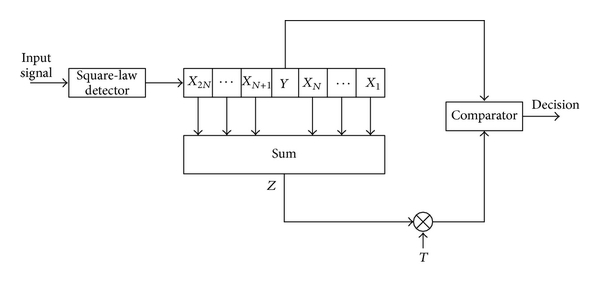
\includegraphics[scale=2.2]{Block-diagram-of-CA-CFAR-detector.png}  
  \end{center}
\caption{CA-CFAR Architecture }
\end{figure}

\end{frame}
%\begin{frame}[t]
%\frametitle{METHrmance degradation in presence of interfering target in reference wODOLOGY(Cont..)}
% \title{Write Operation}

%\textbf{\underline{CFAR Processor Architecture}}
%\vspace{8mm}
%\begin{figure}
 %\begin{center}
   %\includegraphics[scale=0.47]{q.png}  
  %\end{center}
%\caption{CFAR Processor Architecture[7]}
%\end{figure}
%\end{frame}
\begin{frame}[t]
\frametitle{METHODOLOGY(Cont..)}
\textbf{\underline{CA-CFAR Block Diagram}}
\vspace{8mm}
\begin{figure}
 \begin{center}
   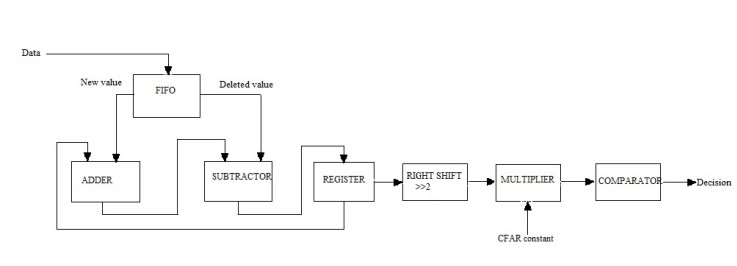
\includegraphics[scale=0.8]{cfar.jpg}  
  \end{center}
\caption{CA-CFAR Block Diagram}
\end{figure}
\end{frame}
\begin{frame}[t]
\frametitle{METHODOLOGY}
\textbf{\underline{Ordered Statistics CFAR}}
\vspace{3mm}
    \begin{itemize}
     \vspace{0.4cm}
     \item OS‐CFAR had been developed to compensate for
         much of CA‐CFAR’s pitfalls.
     \vspace{0.4cm}
     \item Rather than taking the arithmetic mean of adjacent cells.

       \vspace{0.4cm}
       \item OS‐CFAR ranks the N adjacent cells from smallest to largest and multiplies the kth largest cell to the appropriate threshold multiplier to set the threshold level.
       
\end{itemize}
\end{frame}
\begin{frame}[t]
\frametitle{METHODOLOGY(Cont..)}
\textbf{\underline{Ordered Statistics CFAR}}
\vspace{8mm}
\begin{figure}
 \begin{center}
   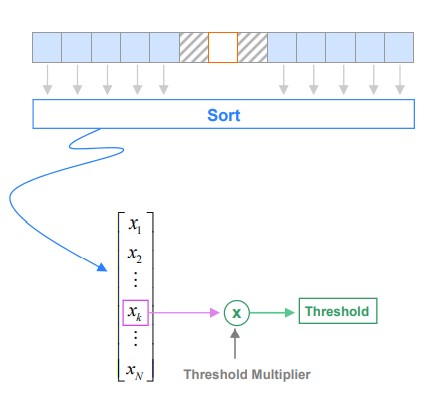
\includegraphics[scale=0.6]{os.jpg}  
  \end{center}
\caption{OS - CFAR Architecture }
\end{figure}

\end{frame}

\section{REQUIREMENTS}
\begin{frame}[t]
\frametitle{REQUIREMENTS}
\begin{itemize}
\vspace{8mm}
\item Software Tools
\begin{itemize}
   \item Xilinx Vivado
   \item Matlab
\end{itemize}
\vspace{1cm}
\item Hardware Tools \begin{itemize}
     \item Xilinx Kintex Ultrascale FPGA
\end{itemize}  
 
\end{itemize}
\end{frame}
\section{SIMULATION RESULTS }
\begin{frame}[t]
\frametitle{SIMULATION RESULTS }
\textbf{\underline{Matlab Results}}\\

     \begin{figure}[h!]
  \begin{center}
   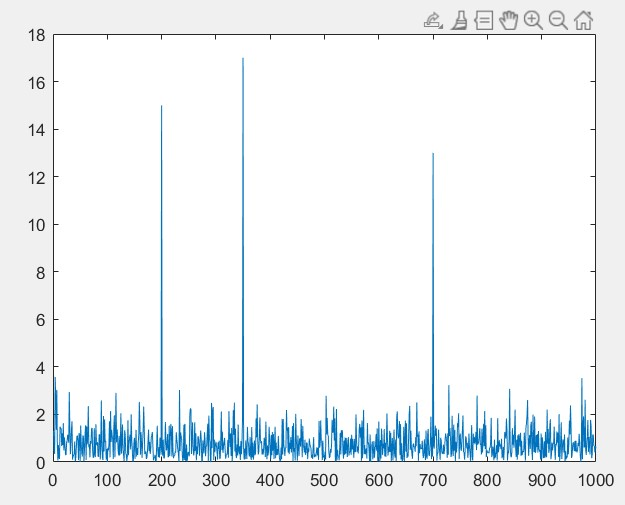
\includegraphics[scale=0.5]{sim.jpg}
    \end{center}
    \caption{Noise Generation (Noise + Target)}
%\label{PFA Computation}
  \end{figure}
\end{frame}
\begin{frame}[t]
\frametitle{SIMULATION RESULTS }
\textbf{\underline{CFAR Detector On Noise}}
     \begin{figure}[h!]
  \begin{center}
   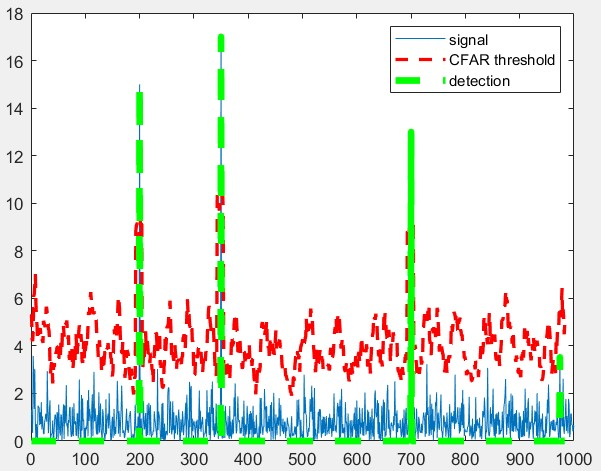
\includegraphics[scale=0.55]{sim2.jpg}
    \end{center}
    \caption{Detection using CA CFAR}
%\label{PFA Computation}
  \end{figure}
\end{frame}
\begin{frame}[t]
\frametitle{SIMULATION RESULTS }
\textbf{\underline{VIVADO Simulation}}
     \begin{figure}[h!]
  \begin{center}
   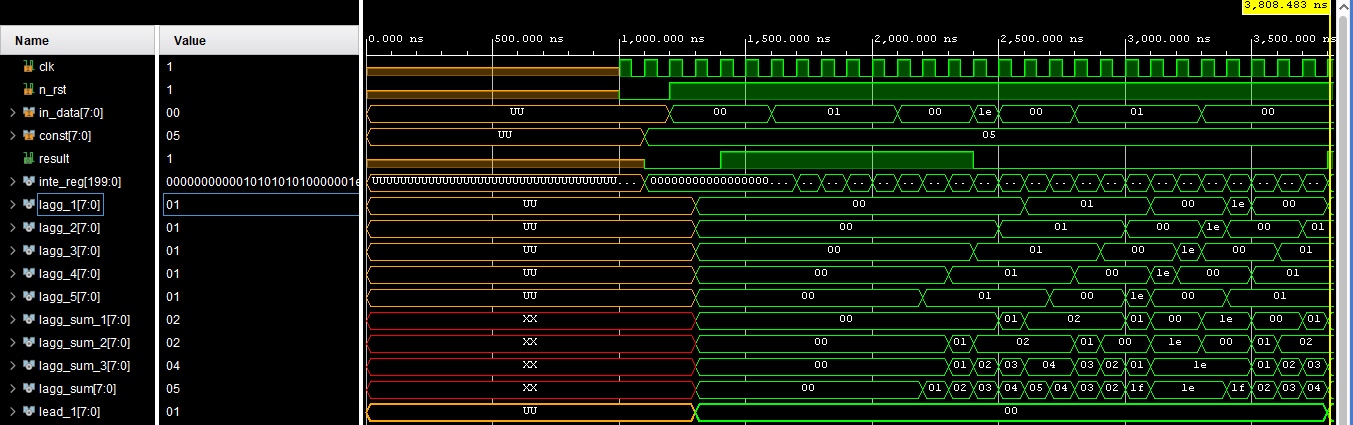
\includegraphics[scale=0.3]{final1.png}
    \end{center}
   
%\label{PFA Computation}
  \end{figure}
   \begin{figure}[h!]
  \begin{center}
   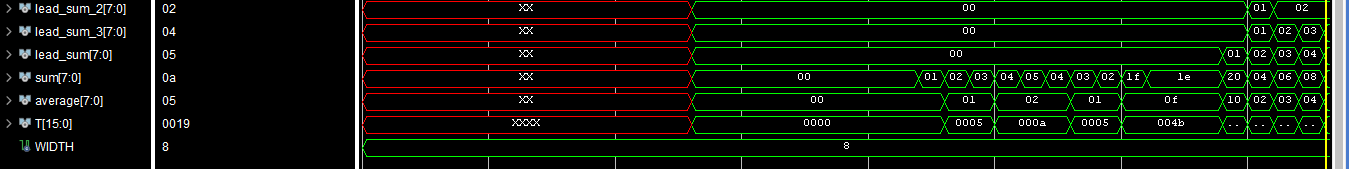
\includegraphics[scale=0.3]{final2.png}
    \end{center}
     \caption{CA-CFAR}
   
%\label{PFA Computation}
  \end{figure}
  
\end{frame}
\begin{frame}[t]
\frametitle{SIMULATION RESULTS }
\textbf{\underline{VIVADO Simulation}}
     \begin{figure}[h!]
  \begin{center}
   \includegraphics[scale=0.3]{OP1.png}
    \end{center}
   

  \end{figure}
   \begin{figure}[h!]
  \begin{center}
   \includegraphics[scale=0.3]{OP2.png}
    \end{center}
     \caption{CA-CFAR}
  
  \end{figure}
  
\end{frame}
\begin{frame}[t]
\frametitle{SIMULATION RESULTS }
\textbf{\underline{VIVADO Simulation}}
   \begin{figure}[h!]
  \begin{center}
   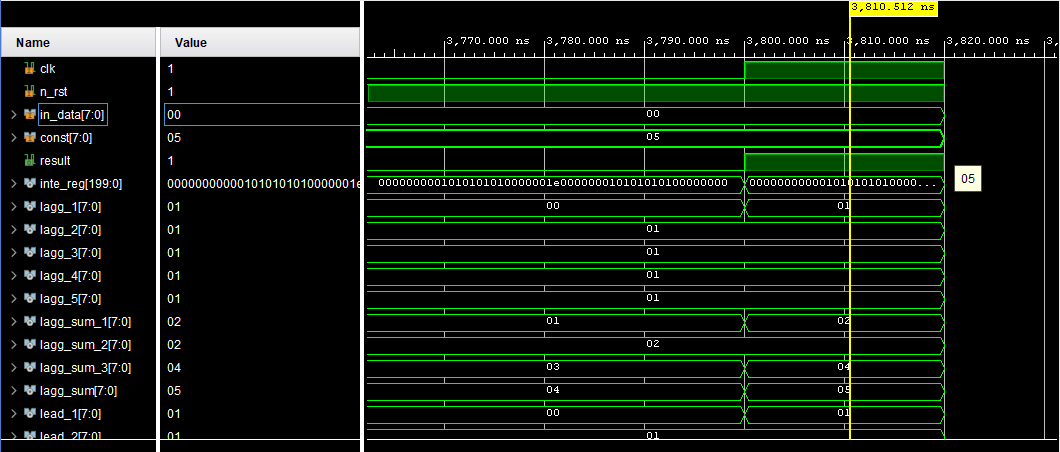
\includegraphics[scale=0.4]{result.png}
    \end{center}
     \caption{CA-CFAR}
  
  \end{figure}
  
\end{frame}


\section{CONCLUSION}
\begin{frame}[t]
\frametitle{CONCLUSION}
 \begin{itemize}
 \vspace{1cm}
     \item The CFAR is a technique being used in detection process stage to keep the false alarm at
an acceptable level.
\vspace{0.4cm}
     \item CA-CFAR and OS-CFAR algorithms are discussed here.
     \vspace{0.4cm}
     \item In CA-CFAR threshold is calculated by multiplying the average value with a constant.
     \vspace{0.4cm}
     \item It is then compared with the value of CUT for target detection.
 \end{itemize}
\end{frame}





\section{REFERENCES}
\begin{frame}[t]
\frametitle{REFERENCES}
%\vskip 1cm

\begin{small}
\item {[1}{]}  Abu, A., & Diamant, R. (2020). CFAR detection algorithm for objects in sonar images. IET Radar, Sonar & Navigation, 14(11), 1757-1766.
\vskip 0.25cm
\item  {[2}{]}Rohling, H. (1983). Radar CFAR thresholding in clutter and multiple target situations. IEEE        transactions on aerospace and electronic systems, (4), 608-621.
\vskip 0.25cm
\item {[3}{]}Saeed, T., Hatem, G., Sadah, J. A., & Ziboon, H. (2020). Design and Implementation of a New CFAR Based on Weighted and Statistical Algorithms.
\item {[4}{]}
 Sambath, P. (2020). Radar Target detection using Cell Evaluation Method for Industrial Safety.
\item {[5}{]}  Kalyan, B., & Balasuriya, A. (2004, April). Sonar based automatic target detection scheme for underwater environments using CFAR techniques: a comparative study. In Proceedings of the 2004 International Symposium on Underwater Technology (IEEE Cat. No. 04EX869) (pp. 33-37). IEEE
\end{small}

\end{frame}
\begin{frame}[t]
\frametitle{REFERENCES}
%\vskip 1cm

\begin{small}

\vskip 0.25cm
\item  {[6}{]} Lawrence, N. B. (1981). Performance Comparison of Cell Averaging and'Greatest-of'Constant False Alarm Rate (CFAR) Methods.
\vskip 0.25cm
\item {[7}{]}SIMIĆ, S., ANDRIĆ, M., & ZRNIĆ, B. (2014). An FPGA based implementation of a CFAR processor applied to a pulse-compression radar system. Radioengineering, 23(1), 73.
\vskip 0.25cm
\item {[8}{]}Analysis of some modified cell-averaging CFAR processors in multiple-target situations. IEEE Transactions on Aerospace and Electronic Systems, (1), 102-114.

\end{small}

\end{frame}
\begin{frame}
\begin{LARGE}
\begin{center}
\textbf{Thank You}
\end{center}
\end{LARGE}
\end{frame}

\end{document}
